\documentclass[11pt,a4paper]{article}

\usepackage[utf8]{inputenc}
\usepackage[T1]{fontenc}
\usepackage{helvet}
\renewcommand{\familydefault}{\sfdefault}
\usepackage[margin=2.2cm, top=2cm, bottom=2cm]{geometry}
\usepackage{graphicx}
\usepackage{xcolor}
\usepackage{booktabs}
\usepackage{float}
\usepackage{caption}
\usepackage{amsmath}
\usepackage{hyperref}
\usepackage{fancyhdr}
\usepackage{tikz}
\usepackage{enumitem}
\usepackage{tabularx}

\definecolor{bigorange}{RGB}{255,130,0}
\definecolor{biggrey}{RGB}{60,60,60}

\hypersetup{colorlinks=true, linkcolor=bigorange, urlcolor=bigorange}

\pagestyle{fancy}
\fancyhf{}
\renewcommand{\headrulewidth}{0.5pt}
\renewcommand{\headrule}{\hbox to\headwidth{\color{bigorange}\leaders\hrule height \headrulewidth\hfill}}
\fancyhead[L]{\small\color{biggrey} Banco BIG $|$ Rates Research}
\fancyhead[R]{\small\color{biggrey} May 2026}
\fancyfoot[C]{\small\color{biggrey}\thepage}

\begin{document}

% COVER
\thispagestyle{empty}
\begin{tikzpicture}[remember picture, overlay]
    \fill[bigorange] (current page.north west) rectangle ([yshift=-9cm]current page.north east);
    \fill[white, opacity=0.15] ([yshift=-3cm]current page.north west) -- ([yshift=-7cm]current page.north west) -- ([yshift=-5cm]current page.north east) -- ([yshift=-1cm]current page.north east) -- cycle;
    \fill[bigorange] ([yshift=1.5cm]current page.south west) rectangle (current page.south east);
\end{tikzpicture}

\vspace*{1cm}
\begin{center}
    
\includegraphics[width=4.5cm]{../Logo-BIG.png}
\end{center}

\vspace{3.5cm}

\begin{center}
    {\Huge\bfseries\color{biggrey} Interest Rate Spillovers}\\[0.4cm]
    {\Huge\bfseries\color{biggrey} to the Brazilian DI Curve}\\[1.0cm]
    {\Large\color{biggrey} 5-Country VAR: US, EU, CA, BR, UK}\\[0.3cm]
    {\Large\color{biggrey} Nelson-Siegel Level, Slope, Curvature}\\[2.0cm]
    {\large\color{biggrey} Rates Research $|$ 5 May 2026}
\end{center}

\vfill
\begin{tikzpicture}[remember picture, overlay]
    \node[anchor=south, yshift=2.0cm] at (current page.south) {
        \color{white}\small\bfseries Banco BIG $|$ Institutional Research
    };
\end{tikzpicture}

\newpage

% PAGE 2: METHODOLOGY & RESULTS
\section*{Methodology: 5-Country VAR on Nelson-Siegel Factors}

We decompose five government yield curves (US, EU, CA, BR, UK) into Level, Slope, and Curvature via Nelson-Siegel ($\lambda=0.10$). A 15-variable VAR(1) is estimated on weekly data (2005--2026, $N=1112$ obs).

\smallskip
\noindent\textbf{Cholesky ordering:} US $\rightarrow$ EU $\rightarrow$ CA $\rightarrow$ UK $\rightarrow$ BR

\smallskip
\noindent Rationale: BR is placed last as the ``receiver'' of interest. US is most exogenous (global reserve currency).

\subsection*{Granger Causality Tests ($\alpha=5\%$)}

\begin{table}[H]
\centering\small
\begin{tabular}{llccc}
\toprule
\textbf{Source} & \textbf{BR Factor} & \textbf{F-stat} & \textbf{p-value} & \textbf{Sig.?} \\
\midrule
    US & Level & 2.36 & 0.070 & Not sig. \\
    US & Slope & 2.64 & 0.048 & \textbf{Sig.} \\
    US & Curvature & 2.60 & 0.050 & Not sig. \\
    EU & Level & 1.25 & 0.290 & Not sig. \\
    EU & Slope & 1.27 & 0.283 & Not sig. \\
    EU & Curvature & 2.50 & 0.058 & Not sig. \\
    CA & Level & 2.94 & 0.032 & \textbf{Sig.} \\
    CA & Slope & 3.24 & 0.021 & \textbf{Sig.} \\
    CA & Curvature & 3.11 & 0.025 & \textbf{Sig.} \\
    UK & Level & 2.13 & 0.095 & Not sig. \\
    UK & Slope & 2.18 & 0.088 & Not sig. \\
    UK & Curvature & 2.57 & 0.053 & Not sig. \\
\bottomrule
\end{tabular}
\end{table}

\begin{figure}[H]
    \centering
    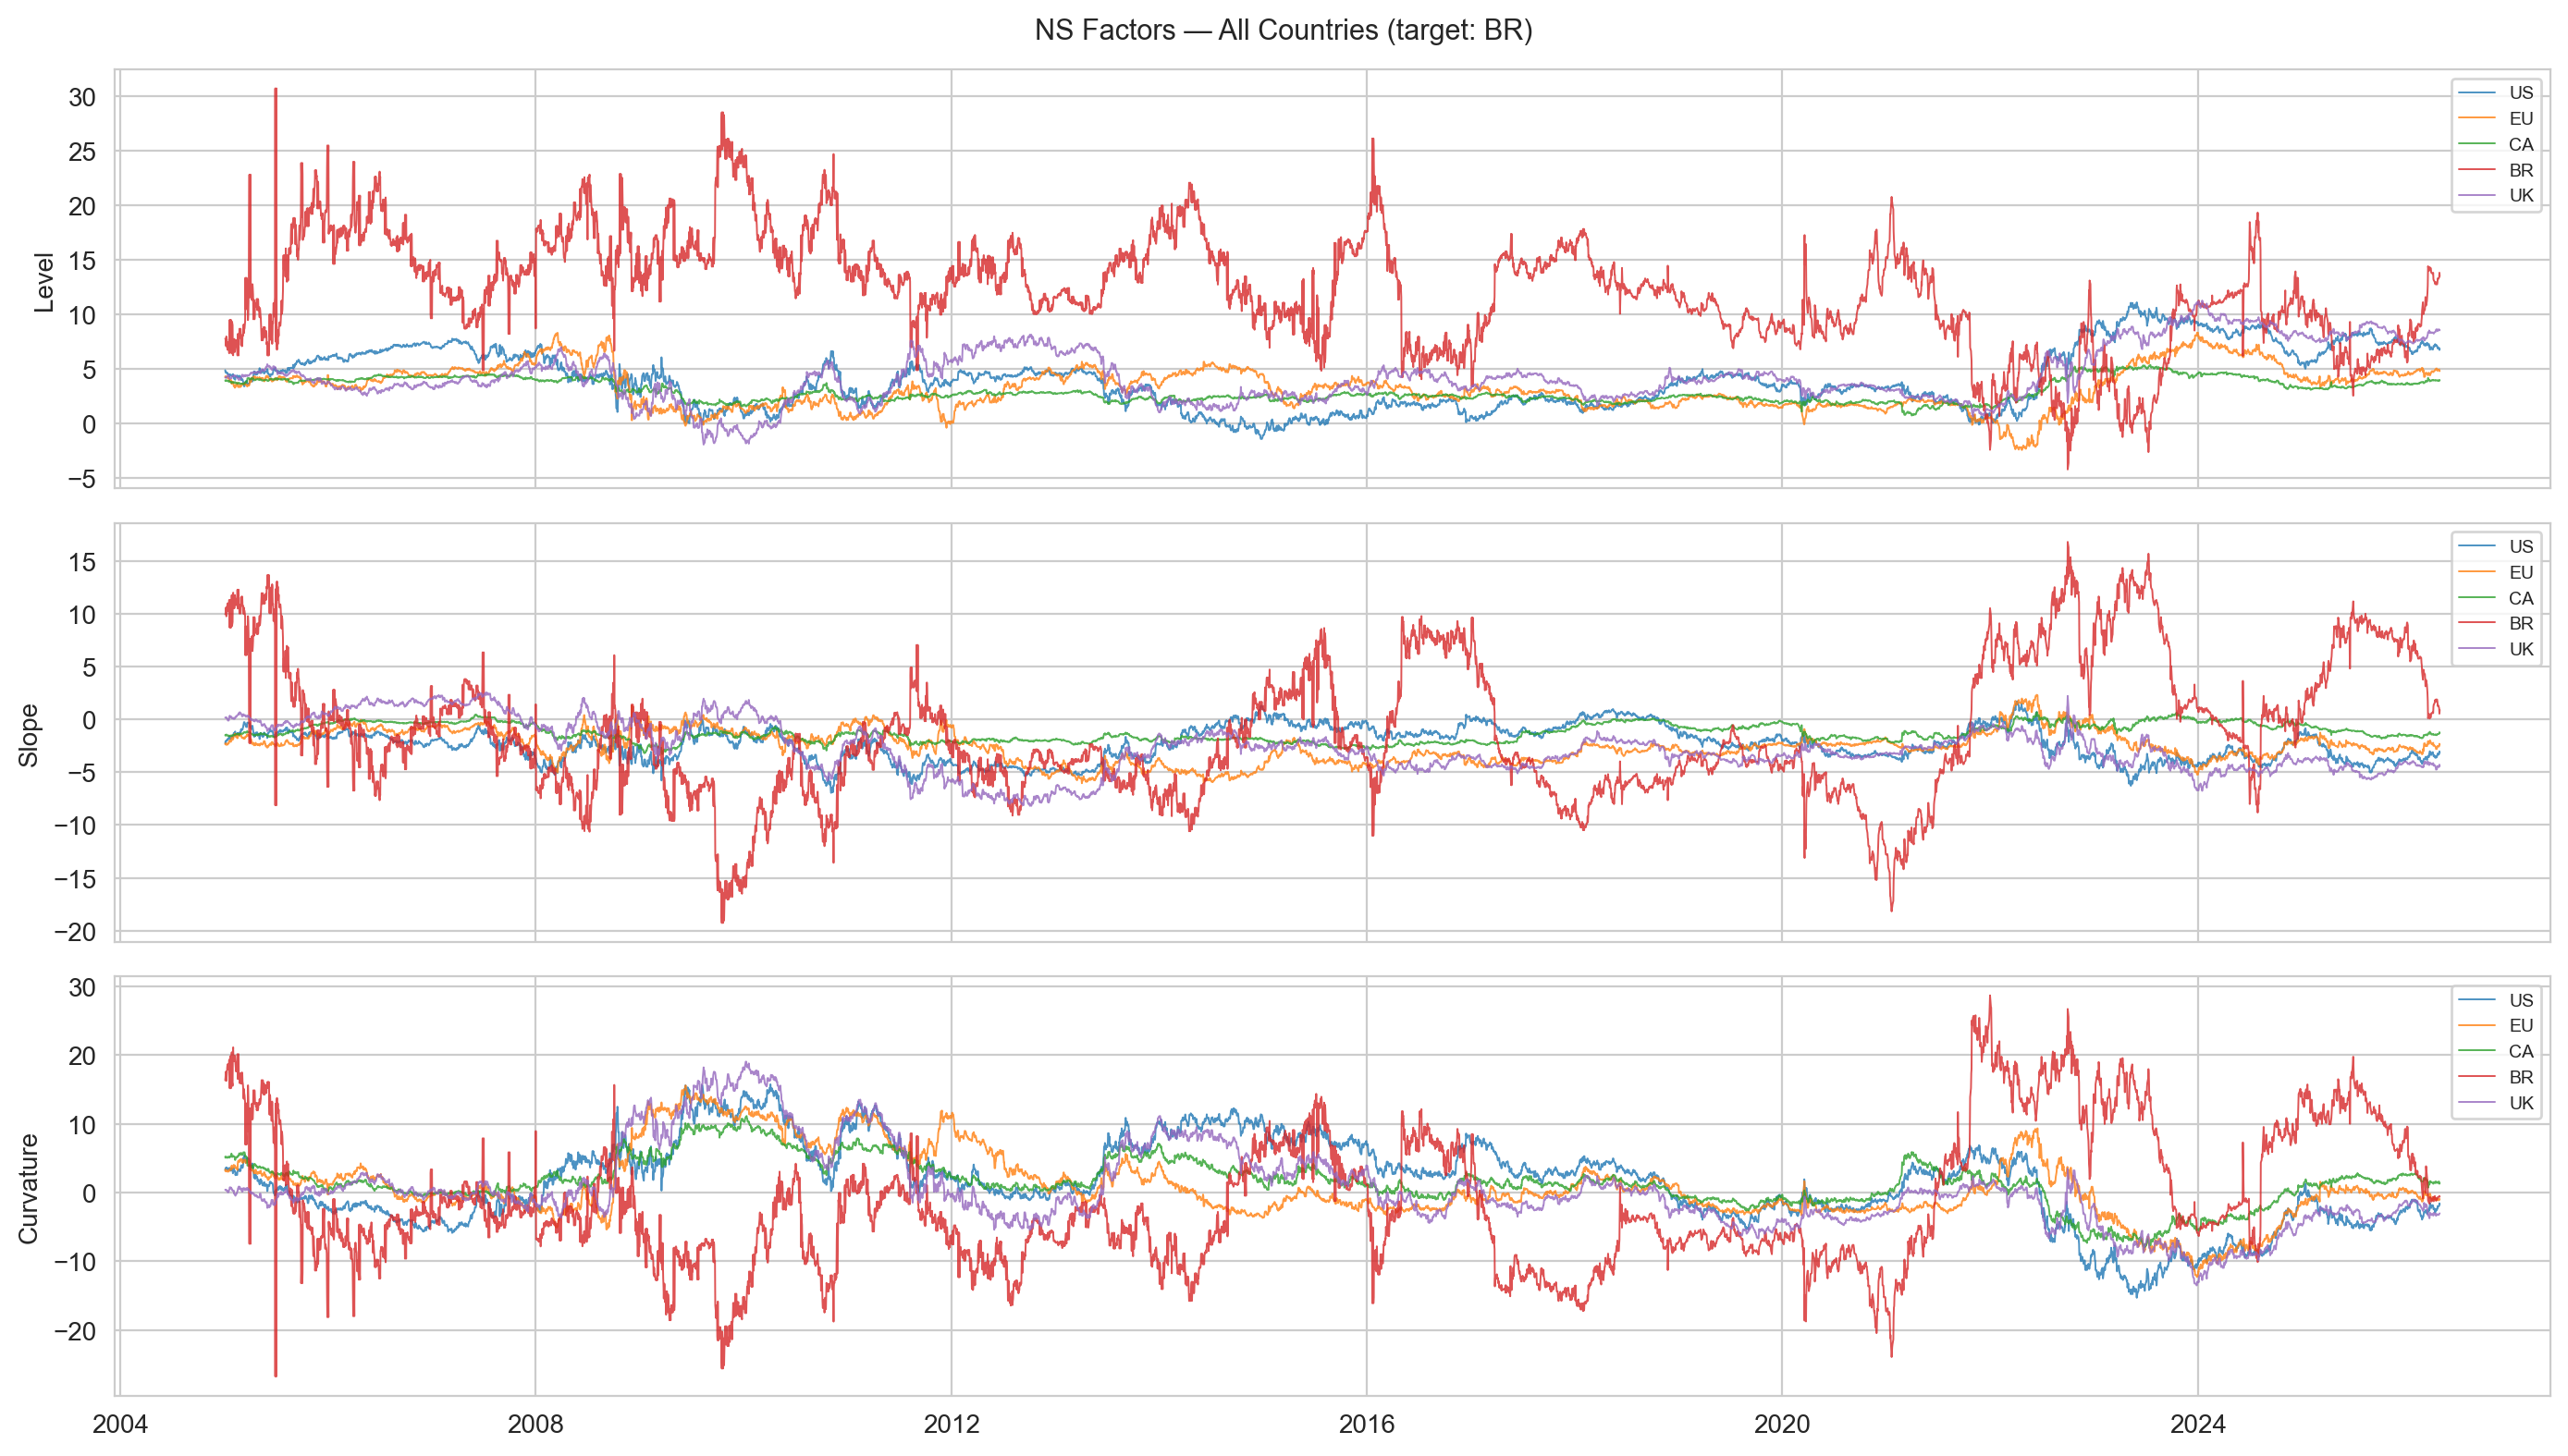
\includegraphics[width=\textwidth]{fig_factors.png}
    \vspace{-0.3cm}
    \caption{\small Nelson-Siegel factors for all 5 countries (2005--2026). BR highlighted as the target curve.}
\end{figure}

\newpage

% PAGE 3: IRFs AND FEVD
\section*{Shock Propagation to Brazil}

\begin{figure}[H]
    \centering
    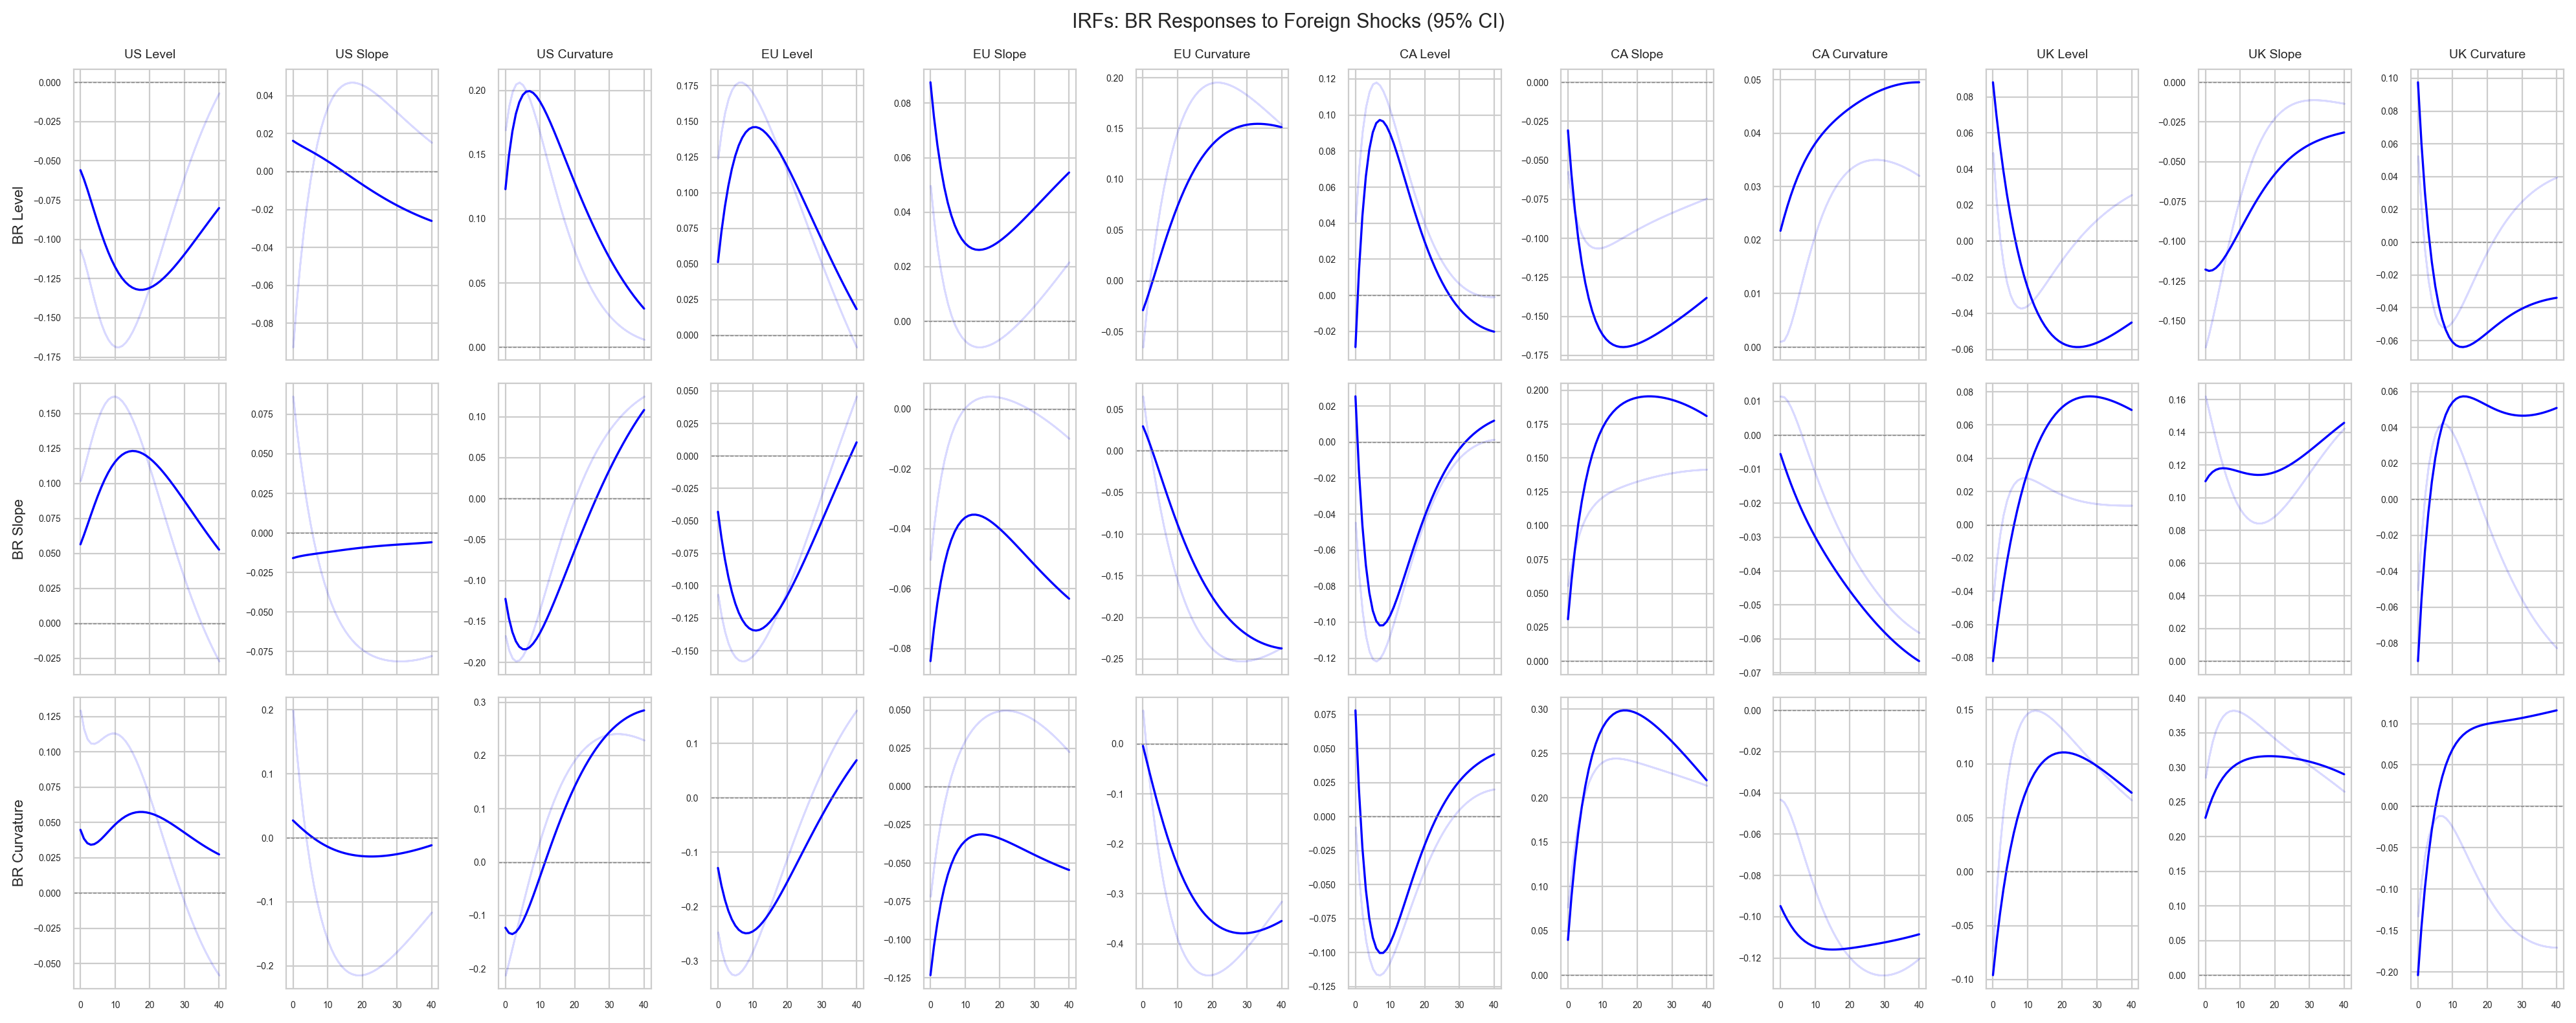
\includegraphics[width=\textwidth]{fig_irf.png}
    \vspace{-0.3cm}
    \caption{\small Orthogonalised IRFs: BR factor responses to foreign shocks over 40 weeks. Blue shading = 95\% bootstrap CI.}
\end{figure}

\subsection*{FEVD at 52-Week Horizon (\% of variance)}

\begin{table}[H]
\centering\small
\begin{tabular}{l c c c c c}
\toprule
 & \textbf{US} & \textbf{EU} & \textbf{CA} & \textbf{BR} & \textbf{UK} \\
\midrule
    BR Level & 7.4 & 7.9 & 7.5 & 74.6 & 2.6 \\
    BR Slope & 4.9 & 10.0 & 7.9 & 72.0 & 5.2 \\
    BR Curvature & 3.6 & 10.0 & 6.0 & 72.0 & 8.4 \\
\bottomrule
\end{tabular}
\end{table}

\begin{figure}[H]
    \centering
    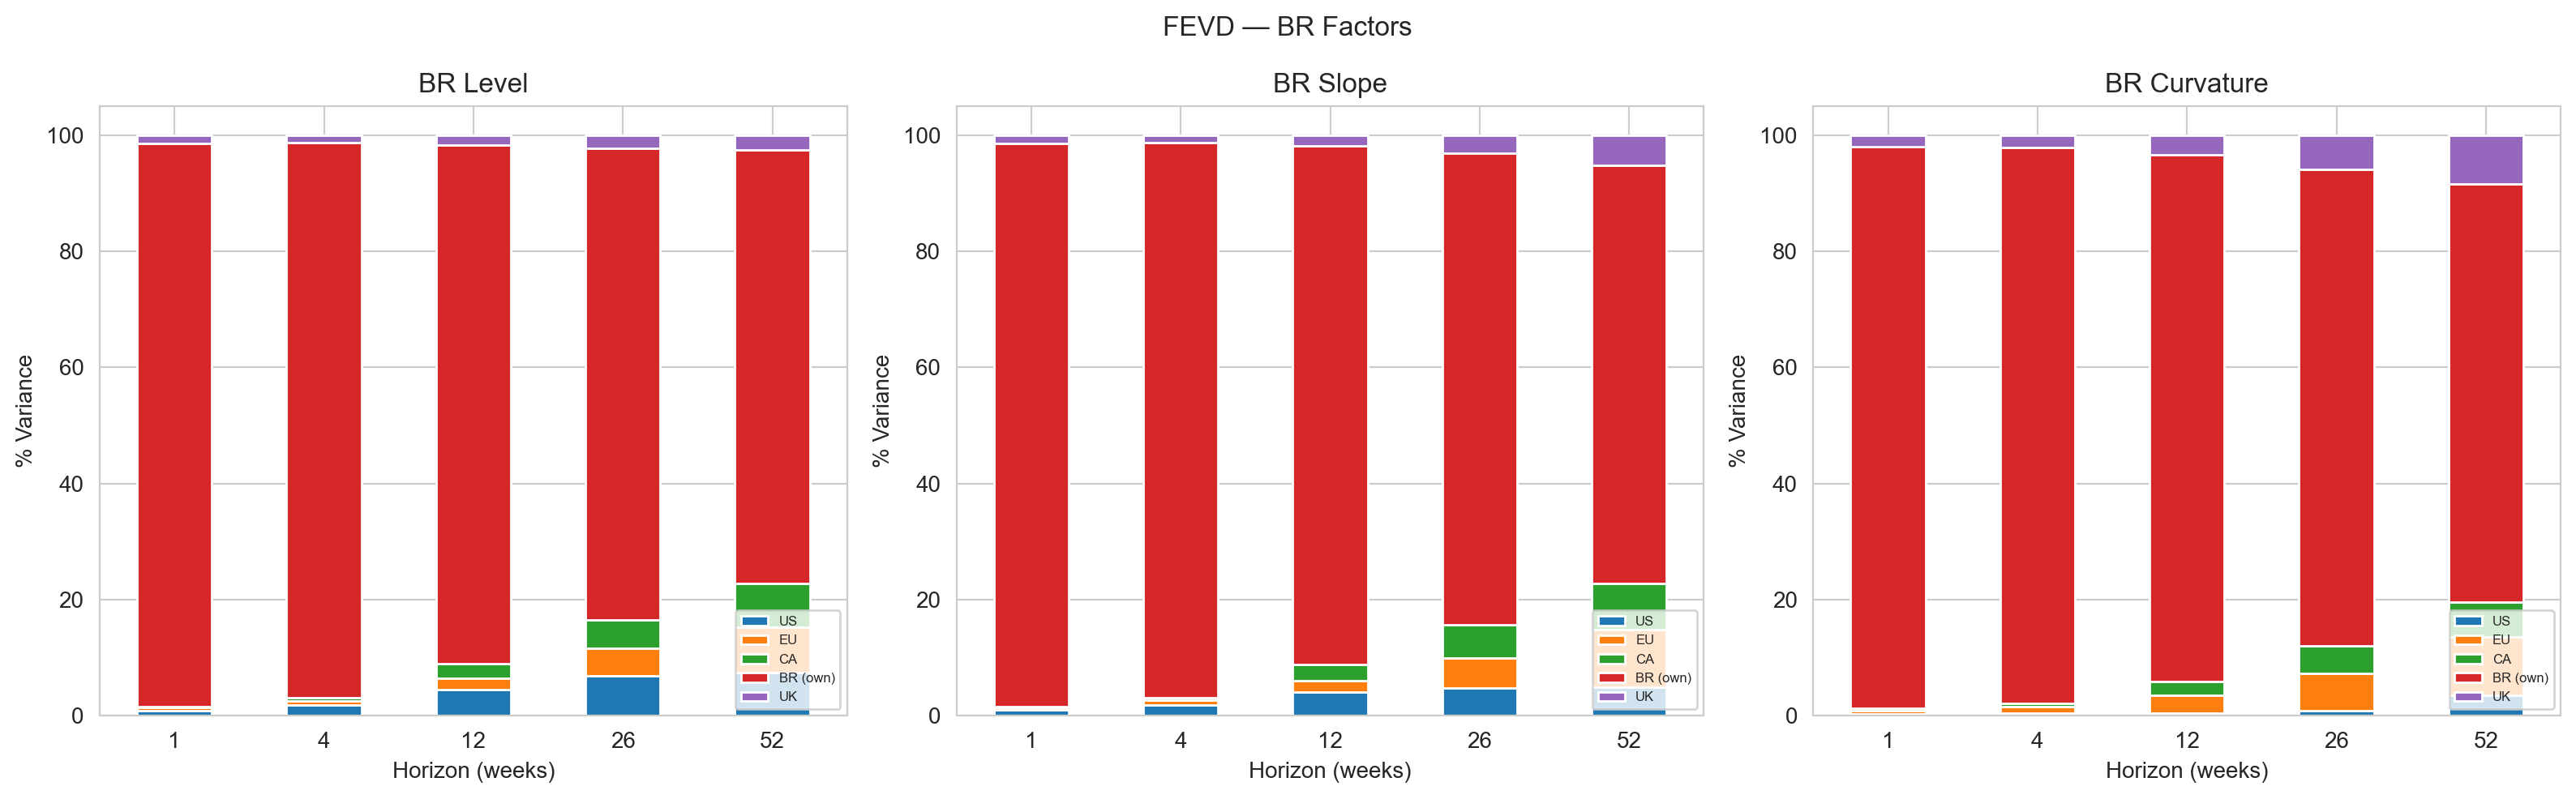
\includegraphics[width=\textwidth]{fig_fevd.png}
    \vspace{-0.3cm}
    \caption{\small FEVD: share of BR factor forecast error variance by source country at horizons 1--52 weeks.}
\end{figure}

\newpage

% PAGE 4: MARKET CONTEXT
\section*{Brazil: Market Context (May 2026)}


\subsection*{Macro \& Fiscal Backdrop}
\begin{itemize}[nosep, leftmargin=1.2em]
    \item \textbf{Inflation:} IPCA at 5.5\% (Mar 2026), above target ceiling (4.5\%). Food and energy pressures persistent.
    \item \textbf{Growth:} GDP grew 2.1\% in 2025. Fiscal stimulus supporting consumption.
    \item \textbf{COPOM:} Selic at 14.75\%, hiked 50bp in March. Forward guidance signals further tightening.
    \item \textbf{Fiscal:} Primary deficit at 0.8\% of GDP. New fiscal framework credibility under pressure.
    \item \textbf{FX:} BRL/USD at 5.80, depreciation adds to imported inflation.
\end{itemize}

\subsection*{Key Drivers Ahead}
\begin{enumerate}[nosep, leftmargin=1.4em]
    \item \textbf{Highest own-determination:} BR curve is the most insular (73\% own-variance across all factors). Domestic monetary policy and fiscal credibility dominate.
    \item \textbf{Limited foreign spillover:} No single foreign block explains more than 10\% of BR variance. Brazil's high carry and idiosyncratic risk dominate.
    \item \textbf{EU as largest foreign driver} ($\sim$10\%): Likely via risk sentiment and European investor flows into EM.
    \item \textbf{Fiscal credibility:} The binding constraint. Any spending cap revision would widen DI rates sharply.
    \item \textbf{Selic path:} Market expects terminal rate of 15.25\%. Any overshoot reprices the entire curve.
\end{enumerate}


\vspace{0.3cm}
\noindent\rule{\textwidth}{0.4pt}
{\footnotesize\color{biggrey} \textbf{Data:} US: FRED (constant-maturity Treasury rates), EU: ECB Statistical Data Warehouse (AAA-rated), CA: Bank of Canada Valet API (benchmark bonds), BR: IPEA/ANBIMA (DI pre-fixed yield curve), UK: Bank of England IADB (nominal spot curve). Model: VAR(1) on weekly NS factors, sample 2005--2026 (1112 obs). This document is for informational purposes only and does not constitute investment advice.}

\end{document}
